% !TeX spellcheck = pl_PL

\chapter{Śledzenie obiektów}
\label{cha:sledzenieObiektow}

Zadanie śledzenia obiektów jest zagadnieniem z dziedziny przetwarzania obrazów. Można podzielić je na dwa główne zadania. Pierwszym jest zachowanie ciągłości analizy ruchu obiektów, czyli zdolność określenia ich pozycji na każdej klatce obrazu z wystarczającą dokładnością. Drugie zadanie dotyczy tylko kamer ruchomych i polega na zdefiniowaniu ich ruchu w~sposób pozwalający zachować śledzony obiekt w polu widzenia. %TOSO 2 średnie. 1. ta "ciągłość analizy" jest dość enigmatyczna, 2. z tym polem widzenie to jest specyficzny przypadek. Może być też śledzenie ze statycznej kamery. Ogólnie trzeba to nieco lepiej opisać.
W praktyce wyznacza się punkt na rejestrowanym obrazie (wartość zadaną) i steruje pozycją oraz orientacją kamery w~taki sposób, by jego odległość od śledzonego obiektu (również reprezentowanego przez punkt) była jak najmniejsza. 
Systemy wizyjne tego typu znajdują zastosowanie m.in. w rozpoznawaniu zachowań ludzi, wykrywaniu kolizji z pieszymi (zaawansowane systemy wsparcia kierowcy -- ang. advanced driver-assistance systems, ADAS), weryfikacji pracy urządzeń przemysłowych czy nawet śledzeniu pojazdów na polu walki.
%TODO 2 rozwinąc skrót ADAS %ODP OK

%---------------------------------------------------------------------------

\section{Rodzaje algorytmów śledzących}
\label{sec:algorytmySledzace}

Algorytmy śledzenia można podzielić na 4 główne kategorie ze względu na metodę identyfikacji obiektu na obrazie. 
Wyróżnia się metody:
\begin{itemize}
	\item różnicowe,
	\item częstotliwościowe,
	\item gradientowe,
	\item korelacyjne,
	\item śledzenia poprzez detekcję,
	\item śledzenia z wykorzystaniem filtrów cząsteczkowych.
\end{itemize}

Ponadto, istnieje również podstawowy podział na sceny stacjonarne i ruchome. 
Wykorzystanie kamery stacjonarnej jest stosunkowo proste w realizacji i nie wymaga dużego nakładu obliczeniowego (do głównych czynności należy separacja tła i segmentacja obiektów ruchomych/pierwszoplanowych). Śledzenie mogłoby być realizowane tylko w obrębie określonej sceny.%TODO 2 no a gdzie to śledznie ? %ODP OK
W~przypadku kamery posiadającej stopnie swobody, pomiędzy obecną i kolejną klatką obrazu zmianie ulec mogą wartości wszystkich pikseli. 
Wyklucza to stosowanie algorytmów opartych o wyodrębnianie tła. 
Dodatkowo, jakikolwiek ruch kamery może zmieniać położenie obiektu i jego wielkość na obrazie -- wymusza to wybór zdecydowanie bardziej złożonych obliczeniowo metod.

\subsection{Algorytmy różnicowe}

Jest to grupa metod, które działają w oparciu o obraz różnicowy, powstały w wyniku odjęcia bieżącego obrazu od poprzedniej klatki lub wcześniej wygenerowanego modelu tła.
Pozwala to na wyodrębnienie obszarów, gdzie nastąpiła zmiana, która zwykle związana jest z ruchem. 
W~celu wyeliminowania szumu (minimalnych zmian w wartościach pikseli) stosuje się progowanie \cite{Rosin}. 
Uzyskuje się maskę binarną -- piksele nieruchome (0) i ruchome (1). 
Analizując taką informację, możliwe jest wyznaczenie nowego położenia obiektu i zdefiniowanie przesunięcia, które nastąpiło pomiędzy klatkami. 

Największą zaletą metod różnicowych jest ich prostota w zrozumieniu oraz implementacji, a~także niska złożoność obliczeniowa. 
Z drugiej jednak strony, tak proste metody bywają zawodne w przypadku większych zakłóceń i ruchu w sąsiedztwie obiektu, błędnie interpretowanego jako właściwe przesunięcie. 
Ponadto, zastosowania tych metod ograniczają się jedynie do obrazów rejestrowanych za pomocą kamery stacjonarnej, co eliminuje je z dalszych rozważań w tej pracy. 

%TODO No dobra. A co jak będą dwa obiekty ? %ODP Pytanie o tę sekcję, czy ogólnie? Jeśli w moim projekciebędą dwie osoby, to algorytm wybierze "bardziej widoczną" i się jej będzie trzymał do czasu zasłonięcia jednej osoby drugą, wtedy się pewnie wysypie.
%TODO 2 - chodziło o tą sekcję... czy ta metoda (tak jak Pan dotarł do opisu) zakłada co się stanie jak będę dwa obiekty. No a uwagę o zachowaniu Pana to trzeba dać gdzieś indziej - jak jeszzce nie ma. %ODP jest w koncepcji, do opisu takiego zachowania nie dotarłem

\subsection{Algorytmy częstotliwościowe}

Metody te opierają się na interpretacji obrazu w dziedzinie częstotliwości. 
Istnieją różne filtry częstotliwościowe, które pozwalają na wykrycie krawędzi -- więc, odpowiednio zaimplementowane, umożliwiają również identyfikację obiektu na kolejnych klatkach wideo. 
Praca w dziedzinie częstotliwości daje możliwość wykrycia przesunięć obiektu, które mogłyby zostać niezauważone w przypadku stosowania pozostałych typów metod. 
Ze względu na swoją wysoką dokładność algorytmy te charakteryzują się nieporównywalnie większą złożonością obliczeniową, związaną z obliczeniem transformaty Fouriera i stosowaniem filtrów częstotliwościowych. %TODO każą jednak opłacić (styl !) %ODP OK 
%TODO 2 -> nie zmienił Pan sformułowania %ODP OK, było 'opłacać', myślałem że chodzi o tę zmianę;)

\subsection{Algorytmy gradientowe}

Działanie wspomnianych metod śledzenia obiektów opiera się na założeniu niewielkich zmian w luminancji (jasności, oświetleniu) oraz niewielkim przesunięciu obiektu pomiędzy kolejnymi klatkami obrazu. 
Istotą tych algorytmów jest znalezienie odpowiedniego przesunięcia obiektu pomiędzy kolejnymi klatkami, tak, aby wskaźnik jakości wynikający z podobieństwa obszarów był zminimalizowany. 
Poszukiwania obszaru można realizować globalnie, bądź na fragmencie będącym otoczeniem śledzonego obiektu. 
Algorytm realizujący obliczenia lokalnie może zawodzić w sytuacjach, gdy przesunięcia są zbyt duże i wykraczają poza obszar poszukiwań, jednak taka metodyka obniża złożoność obliczeniową całego algorytmu i znajduje swoje zastosowania w określonych sytuacjach.
Spośród wielu algorytmów gradientowych stosowanych do śledzenia obiektów, najpopularniejszymi są MeanShift, Camshift oraz KLT \cite{GradientMethods}.  %TODO 2 może \cite do artykułów źródłowych %ODP OK

\subsection{Algorytmy korelacyjne}

Działanie tej grupy algorytmów polega na maksymalizacji funkcji korelacyjnej obliczanej na blokach pikseli.
Podstawowym założeniem jest jeden wspólny kierunek przemieszczenia wszystkich punktów obiektu.
Istotnym dla złożoności i wydajności parametrem przy implementacji tej grupy metod jest określenie rozmiaru obszaru poszukiwań -- w przypadku mniejszych, problemem bywa przemieszczenie obiektu poza obszar; w przypadku tych większych istnieje ryzyko znalezienia maksimum funkcji korelacyjnej, które nie odpowiada obiektowi. 
Zaletą metod korelacyjnych jest jednak mniejsza wrażliwość na zachodzące na siebie obiekty, co umożliwia śledzenie bardziej złożonych ruchów 
Stosuje się je często, gdy obliczanie pochodnych (dla metod gradientowych) byłoby utrudnione -- przykładowo w przypadku gwałtownego ruchu obiektu lub niewystarczającej częstotliwości próbkowania sygnału wideo. 
Jedną z najbardziej popularnych metod korelacyjnych jest BMA (ang. block-matching algorithm), często używana w kompresji wideo \cite{Aroh}. %TODO 2 rozwinąć skrót. %ODP OK

\subsection{Algorytmy śledzenia przez detekcję}

Działanie tej grupy algorytmów polega na niezależnym wykrywaniu określonych obiektów w kolejnych klatkach obrazu. 
Detekcja jest oparta na ekstrakcji kilku cech charakterystycznych obiektu, na przykład opisujących kształt.
W kolejnym etapie tak stworzony deskryptor jest klasyfikowany jako poszukiwany obiekt lub odrzucany. 
Istotną wadą tych metod śledzenia jest duża wrażliwość na zmianę odległości od obiektu -- rozwiązuje się ten problem poprzez analizę kilku przeskalowanych obrazów, jednak podnosi to ogólną złożoność obliczeniową ekstrakcji cech. 
Odrębną kwestią są parametry klasyfikatora -- uzyskiwane w procesie uczenia i mocno wpływające na efekty działania tych metod.
W skład tej grupy wchodzą m.in. algorytmy HOG (ang. Histogram of Oriented Gradients), SIFT (ang. Scale-Invariant Feature Transform) oraz SURF (ang. Speeded-Up Robust Features) \cite{RHOG}. %TODO 2 rozwinąć skróty %ODP OK

%TODO kolejna kwestia to jednak wypadałoby powołać się na jakąś literaturę na podstawie, której Pan to opisał.
%TODO 2 tych odnośników Pan nie dodał ? %ODP ten komentarz był do wpisu wyżej, algorytmy śledzenia przez detekcję opisałem dopiero w ostatnim czasie. No ale mogłem coś zacytować przy okazji.

\subsection{Algorytmy śledzenia wykorzystujące filtry cząsteczkowe}

Idea działania tej grupy metod polega na przedstawieniu pozycji obiektu za pomocą zbioru losowych próbek (cząsteczek). 
Każda z nich związana jest z prawdopodobieństwem obecności obiektu w pozycji reprezentowanej przez tę cząsteczkę. 
Po otrzymaniu nowej klatki obrazu, cząsteczkom są przypisywane wagi na podstawie zgodności predykcji. W najprostszym przypadku jest to efekt porównania histogramów interpretowanych jako rozkłady gęstości prawdopodobieństwa. %TODO 2 zbyt "nieprecyzyjne" musi tu Pan doczytać. Natomiast w najprostszym przypadku sprowadza się to do porównywnia histogramów.. (jako rozkładu prawdodopobieństwa). %ODP OK
Następnie cząsteczki z ,,odpowiednio'' dobrym wynikiem są pomnażane, natomiast te o złych parametrach są eliminowane z dalszych obliczeń.
Wydajność tej grupy algorytmów w~dużej mierze zależy od liczby zdefiniowanych cząsteczek, przy czym parametr ten ma również istotny wpływ na skuteczność śledzenia.

%Nie wiem, czy mój opis jest do końca poprawny.
\subsection{Podsumowanie}

Ostatecznie w realizacji projektu postanowiono zaimplementować algorytm gradientowy: MeanShift i metodę śledzenia przez detekcję: HOG+SVM.
O takim wyborze zadecydowała możliwość wykorzystania obu rozwiązań dla obrazu pochodzącego z kamery ruchomej, co w~przypadku pracy drona było decyzją naturalną. 
Mimo, że MeanShift jest algorytmem iteracyjnym (kryterium zakończenia obliczeń stanowi limit iteracji, bądź uzyskanie określonej dokładności), to odpowiednie zaprojektowanie modułu obliczeniowego w FPGA pozawala przetwarzać obraz w czasie rzeczywistym, tj. ukończyć obliczenia dla aktualnej klatki przed rozpoczęciem przetwarzania kolejnej - tak szybko, jak tylko uzyska się na jej temat komplet informacji. 
Metoda ta charakteryzuje się dobrymi wynikami w przypadku obiektów zmieniających orientację -- jest to szczególnie przydatne w sytuacji, gdy miejscem umiejscowienia kamery jest dron -- maszyna podatna na podmuchy wiatru zmieniające chwilowo jej orientację względem obiektu. 

Z kolei zastosowanie algorytmu HOG+SVM jest związane z rozpoznaniem kształtu człowieka, co będzie stanowić podstawową metodę potwierdzenia jego obecności na obrazie. Dodatkową korzyścią wynikającą z implementacji algorytmu HOG+SVM jest możliwość pierwotnej detekcji postaci, na podstawie której uruchomiony zostanie system śledzenia. 
Ponadto, jednoczesna analiza kilku przeskalowanych obrazów na danym obszarze pozwoli wybrać najlepszy wynik i określić na tej podstawie odległość kamery od celu.  %TODO kompensowanie głębi- usunąć. Natomiast tą rolę trzeba opisać lepiej. Ale to i tak będzie miało sens tylko, jak wcześniej (zgodnie z sugestią) przecyzjie zostanie opisana koncepcja. Rola algorytmu HOG jest dwojaka. Odległość, ale też rozumiem inicjalizacja/re-inicjalizacja mean-shift (metody się uzupełniają) - no przynajmniej w teorii. %ODP Opisano
%TODO 2 no mógłby Pan lepiej rolę tego HOG opisać. %ODP OK
%Poprawność działania systemu wbudowanego będącego połączeniem obu algorytmów została potwierdzona testami, które zostały przeprowadzone na modelu programowym oraz na symulacjach kodu System Verilog. %TODO to zdanie to do innej cześci pracy. Tu na razie koncepcja. %ODP OK

Oba algorytmy były wcześniej implementowane w układach rekonfigurowalnych w niezależnych projektach \cite{Mazur},\cite{Patel}, \cite{Drozdz}.
%TODO Można też dodać, że oba algorytmy były wcześniej implementowane w FPGA (literatura). %ODP OK

\section{Algorytm MeanShift}

MeanShift jest algorytmem zaprezentowanym po raz pierwszy w 1975 roku przez K. Fukunagę i L. Hostetlera \cite{Fukunaga}. 
Jest to metoda znajdowania maksimum rozkładu gęstości na pewnym ograniczonym obszarze. 
Iteracyjny charakter algorytmu pozwala aktualizować położenie obszaru, przemieszczając go w kierunku maksimum i rozpoczynając ponownie analizę.

Z czasem stwierdzono, że MeanShift może znaleźć zastosowanie w systemach wizyjnych. Dysponując bowiem obszarem na obrazie, w którym znajduje się śledzony obiekt, należy zapamiętać jego funkcję gęstości prawdopodobieństwa w postaci histogramu barw.
Pełnić on będzie rolę wzorca, z którym porównywane będą histogramy obszarów z kolejnych klatek obrazu (kandydaci).
 %TODO 2 ??? to jest jakieś niejasne. %ODP OK
Funkcje gęstości prawdopodobieństwa są obliczane z uwzględnieniem jądra o zdefiniowanej postaci, którego wagi faworyzują wartości pikseli w centrum obszaru. 
Dzięki właściwemu doborowi jądra algorytm z odpowiednią zbieżnością znajduje przesunięcie odpowiadające maksimum rozkładu gęstości (podobieństwa). Następnie obszar śledzenia zmienia swoje położenie zgodnie z obliczonym wektorem MeanShift, by dysponując nowym zestawem pikseli, możliwe było rozpatrzenie nowego kandydata.
%TODO TU by się przydało jakieś wprowadzanie i podanie źródła z literatury. %ODP OK
%TODO 2 Proszę to sobie przeczytać i jednak jaśniej/prościej opisać. %ODP OK

\subsection{Konwersja przestrzeni barw RGB->HSV}
\label{sec:rgb2hsv} 

%TODO Opis mean-shift jest ~ poprawny, ale taki dość trudny do zrozumienia. Na początku trzeba w kilku zadaniach opisać o co chodzi - tak jak jest to na tym schamcie blokwoym i potem uszczegółowić. Proszę też jeszcze raz sprawdzić wzory. %ODP OK

Algorytm MeanShift użyty w procesie śledzenia wykorzystuje rozkład prawdopodobieństwa wybranej cechy na obrazie -- w tym wypadku barwy. 
Jest to składowa H z przestrzeni barw HSV (ang. \textit{Hue, Saturation, Value}). 
Domyślną przestrzenią do rejestracji i zapisu obrazów jest jednak RGB, zatem wymagana jest jej konwersja. 
O ile przestrzeń RGB reprezentowana jest przez sześcian określony parametrami 3 kolorów: czerwonego, zielonego i niebieskiego, to przestrzeń barw HSV opisywana jest przez stożek. 
Jego podstawą jest koło, którego kąt opisuje barwę (H -- \textit{Hue}).
Kolor czerwony jest reprezentowany przez kąty $0$\si{\degree} (lub $360$\si{\degree}), zielony przez kąt $120$\si{\degree}, a kolor niebieski przez $240$\si{\degree}. 
Promień koła barw opisuje nasycenie koloru (S -- \textit{Saturation}), zaś za moc światła białego, czyli jasność (V -- \textit{Value}) odpowiada wysokość stożka. 
Model HSV jest lepiej powiązany ze sposobem w jaki postrzega ludzki narząd wzroku, dla którego wszystkie barwy są światłem odbitym od obiektów.
Rysunek \ref{fig:HSV_cone} przedstawia interpretację graficzną składowych przestrzeni HSV na stożku.

\begin{figure}[h]
	\centering
	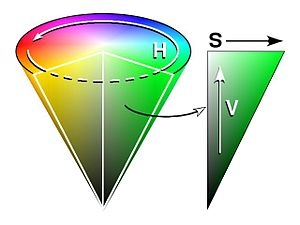
\includegraphics[width=6cm]{2_HSV.jpg}
	\caption{Stożkowa przestrzeń barw modelu HSV \cite{HSV}} 
	\label{fig:HSV_cone}
\end{figure}

Poniższe wzory opisują sposób wyznaczenia poszczególnych składowych przestrzeni HSV w oparciu o RGB \cite{Kryjak}. 
Wymagają one kilku względnie złożonych operacji dzielenia.

\begin{equation}
\label{HSV_first}
V=max(R,G,B)
\end{equation}

\begin{equation}
S=\begin{cases}
\frac{V-min(R,G,B)}{V}, & V\neq0 \\
0, & V=0
\end{cases}
\end{equation}

\begin{equation}
\label{HSV_last}
H=\begin{cases}
	0, & \text{jeśli } V-min(R,G,B)==0 \\
	\frac{60(G-B)}{V-min(R,G,B)}, & \text{jeśli } V==R \\
	\frac{60(B-R)}{V-min(R,G,B)}+120, & \text{jeśli } V==G \\
	\frac{60(R-G)}{V-min(R,G,B)}+240, & \text{jeśli } V==B 
\end{cases}
\end{equation}


\subsection{Wektor MeanShift}
\label{ssec:MS}

Istotą działania algorytmu MeanShift jest wyznaczanie maksimum funkcji gęstości w kolejnych iteracjach. 
Dla określanego obszaru obliczany jest środek ciężkości punktów, których nagromadzenie wskazuje na większy stopień podobieństwa rozpatrywanego obszaru z oryginałem (wzorcem). 
Do nowego środka ciężkości zostaje przesunięte aktualne położenie centrum obszaru po zakończeniu iteracji algorytmu. %TODO 2 to x2 środka tak średnio zręczne. %ODP OK

To przesunięcie nosi nazwę \textit{wektora MeanShift}, który dla zbioru \textit{n} punktów $\{x_{i}\}_{i=1..n}$ oraz środka obszaru w punkcie $y_0$ może zostać zapisany jako:

\begin{equation}
\label{eq:ms1}
M(y)=\bigg[\frac{1}{n}\mathlarger{\sum\limits_{i=1}^{n}}x_i\bigg]-y_0
\end{equation}

Prostota wzoru \eqref{eq:ms1} wynika z ujednolicenia wagi dla wszystkich punktów. 
Wprowadzając wagę punktu zależną od jego odległości od środka obszaru -- takiej, która maleje wraz z~oddalaniem się od centrum), wzór \eqref{eq:ms1} można przepisać jako:

\begin{equation}
\label{eq:ms2}
M(y)=\frac{\sum_{i=1}^{n}w_i(y_0)x_i}{\sum_{i=1}^{n}w_i(y_0)}-y_0
\end{equation}
W równaniu \eqref{eq:ms2}, $w_i(y_0)$ są wagami dla poszczególnych punktów.

Rysunek  \ref{fig:ms_vector} ilustruje przykładowe wygenerowanie wektora MeanShift, gdzie niebieskim okręgiem zaznaczono obszar podlegający działaniu algorytmu. 
Wszystkie punkty mają tu jednak identyczną wagę.
\begin{figure}[h]
	\centering
	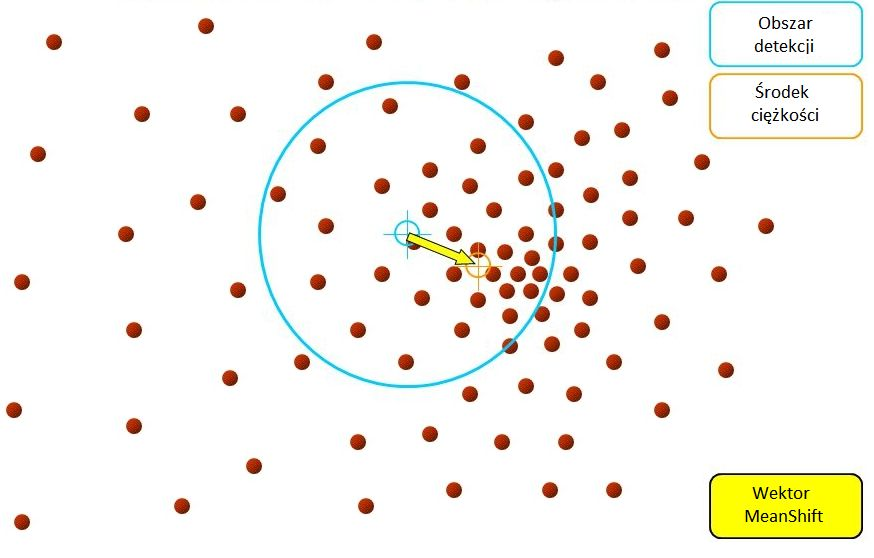
\includegraphics[width=10cm]{2_meanshift.jpg}
	\caption{Graficzna interpretacja wektora MeanShift \cite{Egorov}}
	\label{fig:ms_vector}
\end{figure}


\subsection{Jądro obszaru}

Celem wyznaczenia jądra (ang. kernel) dla obszaru o stałej wielkości jest przypisanie najwyższej wagi punktom, które znajdują się najbliżej środka obszaru. 
Konsekwencją tego jest nadawanie znikomych wag punktom na jego brzegach. 
Postać jądra zwykle przyjmuje klasyczne postacie gęstości rozkładów probabilistycznych: między innymi rozkładu jednorodnego (wagi jednakowe), prostokątnego, Gaussa, Cauchy'ego, Epanechnikova. 
W niniejszej pracy zdecydowano się wykorzystać jądro trójkątne ze względu na jego dobre wyniki i jednoczesną prostotę implementacji, nie bez znaczenia podczas późniejszej realizacji sprzętowej w układzie FPGA. 
Jądro takie można opisać poniższym wzorem:

\begin{equation}
\label{eq:ms3}
K(u)=\begin{cases}
1-\frac{u}{b}, & \text{jeśli }\frac{u}{b}\leq 1 \\
0, & \text{jeśli }\frac{u}{b} > 1
\end{cases}
\end{equation}
gdzie: $u$ jest odległością pomiędzy punktem a środkiem obszaru, a $b$ jest połową jego boku (zakładając, że obszarem jest kwadrat). Rysunek \ref{fig:kernel} przedstawia jądro o wymiarach $100\times 100$ -- w punkcie $(50,50)$ osiąga maksymalną wartość $1$ (natomiast $u=0$).
\begin{figure}[h]
	\centering
	\captionsetup{justification=centering,margin=1cm}
	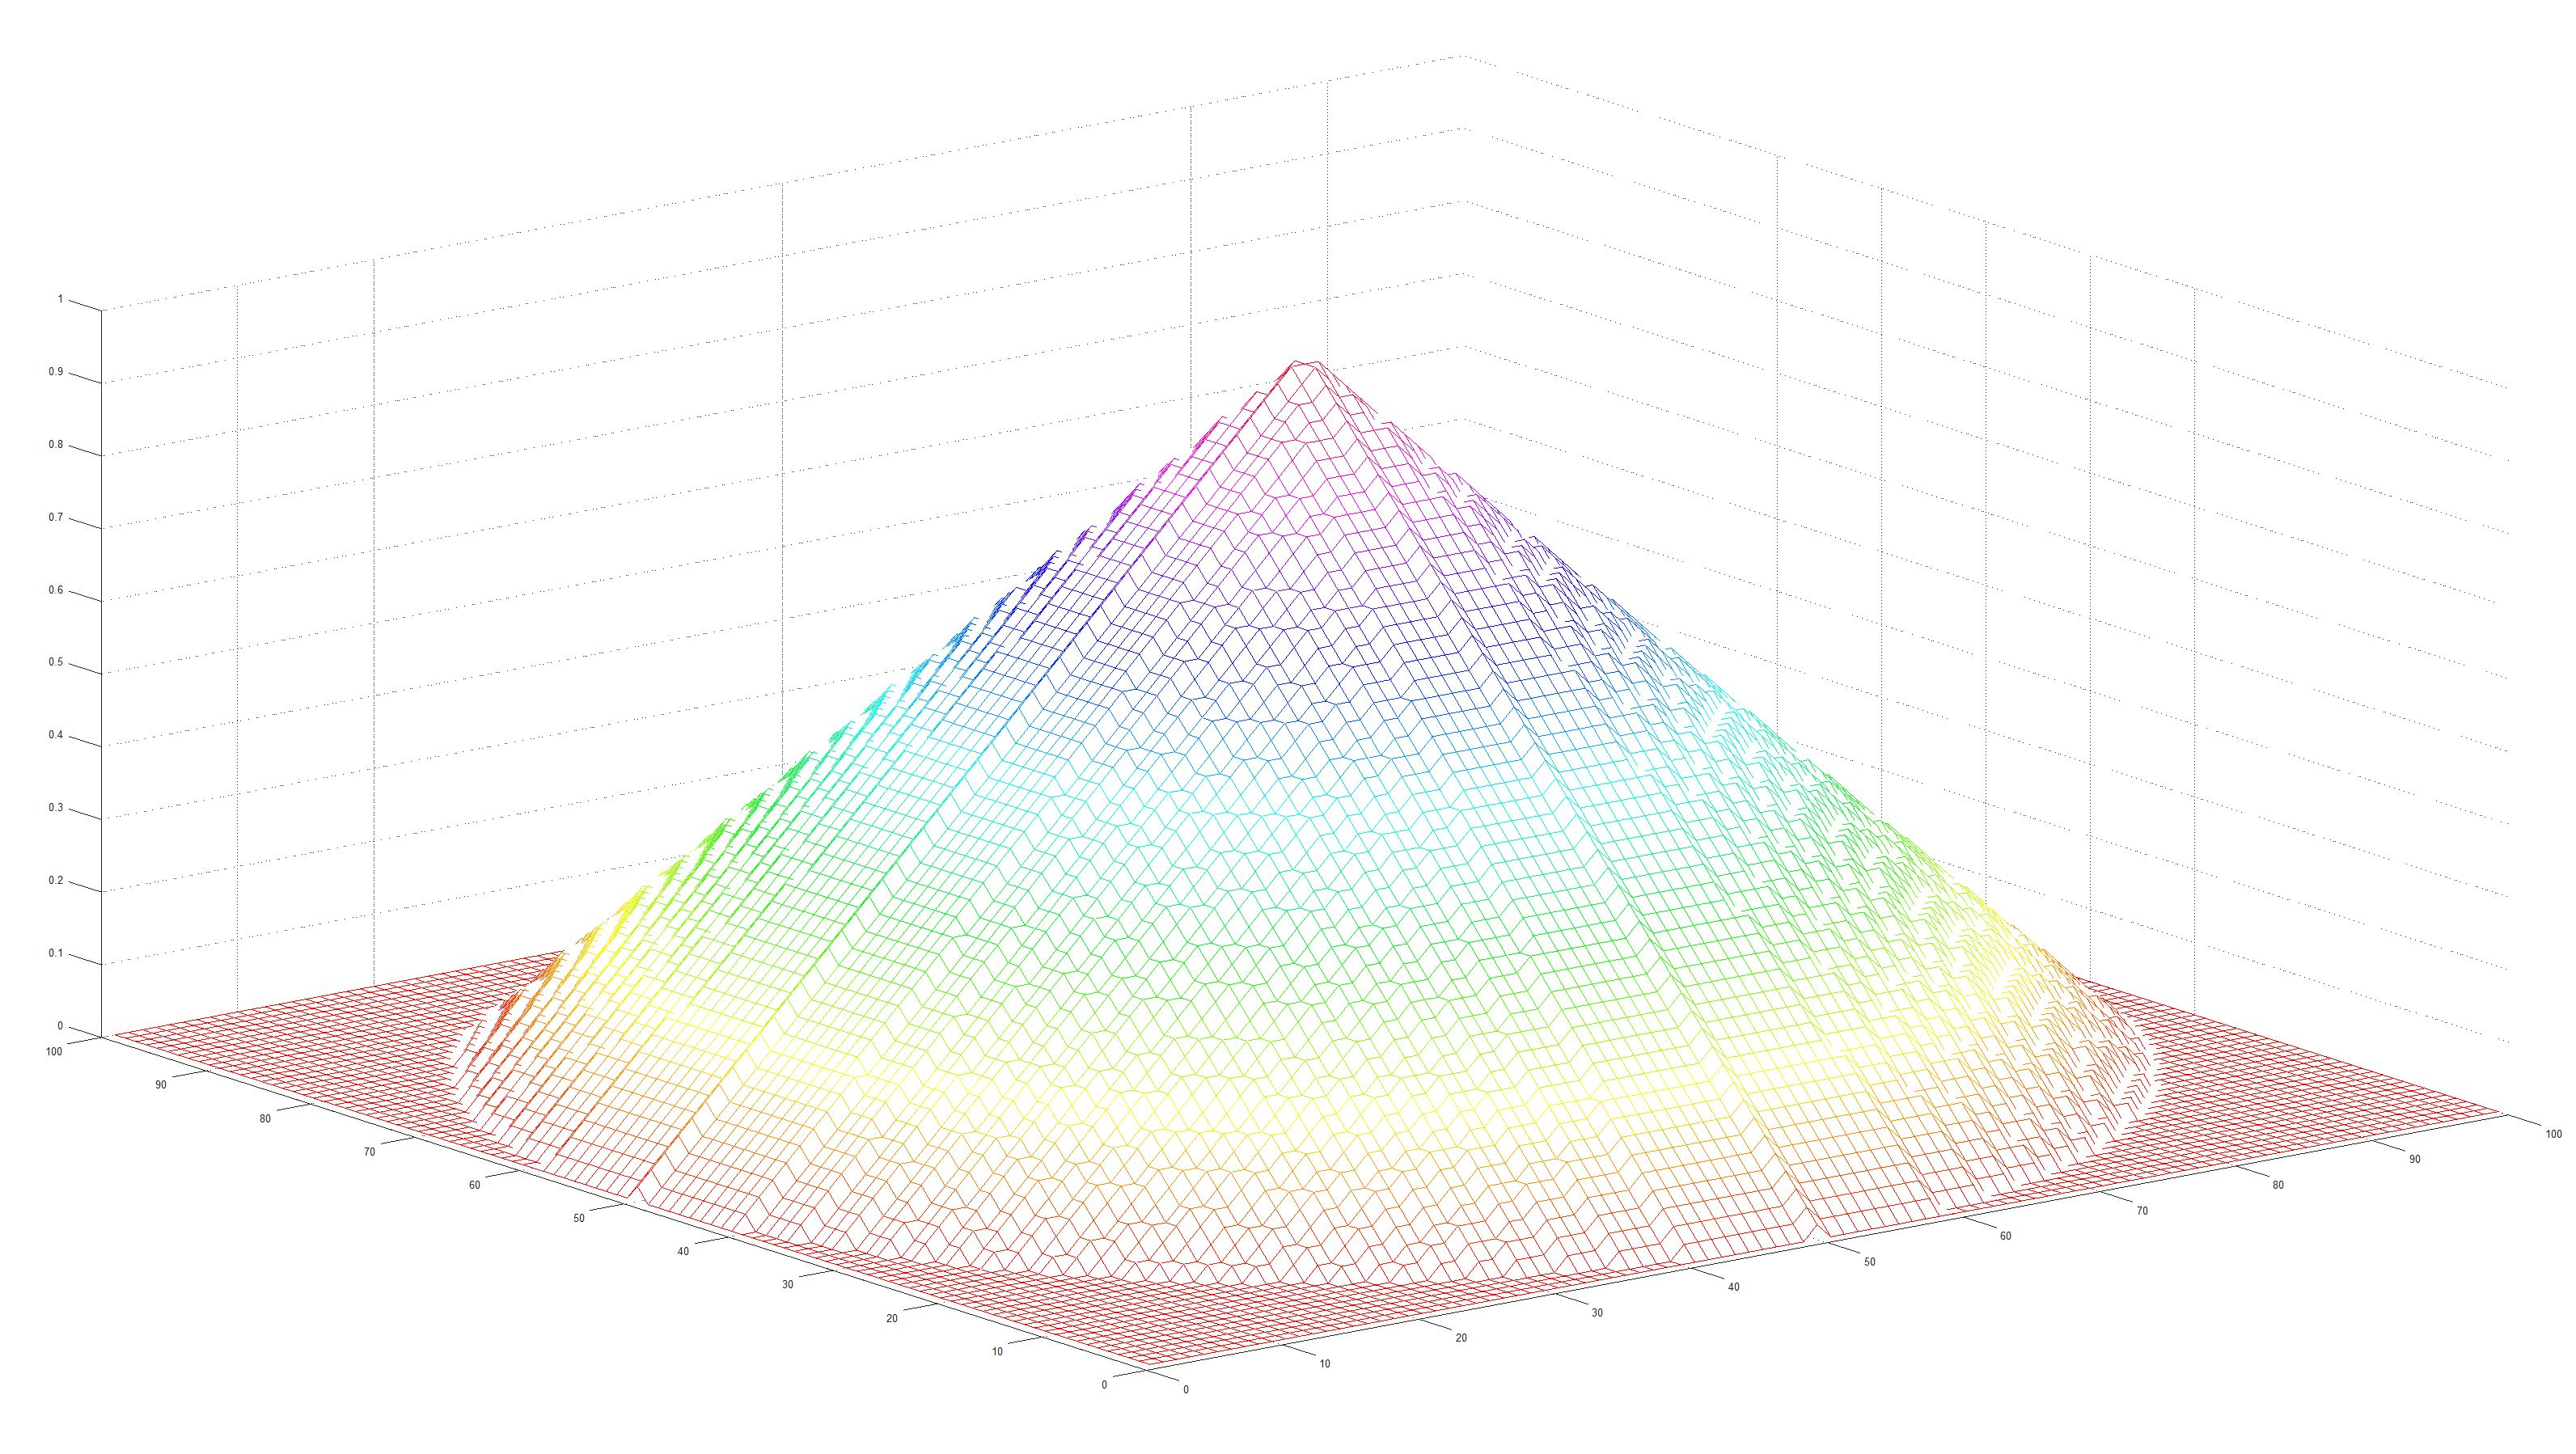
\includegraphics[width=12cm]{2_kernel.jpg}
	\caption{Jądro obszaru o wymiarach $100\times100$ (wygenerowane w programie MATLAB)}
	\label{fig:kernel}
\end{figure}


\subsection{Gęstość jądra}
Mając zbiór $n\times n$ punktów: $\{x_{i},y_{j}\}_{i=1..n,i=j..n}$ z przestrzeni $\mathbb{R}^2$ oraz jądro $K(u)$ dla punktu centralnego $P=(x,y)$ można przedstawić funkcję oszacowania gęstości:

\begin{equation}
f(P)=\frac{1}{n^2}\sum_{i=1}^{n}\sum_{j=1}^{n}K(||P-P'(i,j)||).
\end{equation}
Różniczkując powyższe otrzymuje się:
\begin{equation}
\label{eq:K}
\nabla f(P)=\frac{1}{n^2}\sum_{i=1}^{n}\sum_{j=1}^{n}(P-P'(i,j))K'(||P-P'(i,j)||),
\end{equation}
a po podstawieniu $g(x)$ za $-K'(x)$, wzór \eqref{eq:K} może zostać zapisany jako:
\begin{equation}
\nabla f(x)=\frac{1}{n^2}\sum_{i=1}^{n}\sum_{j=1}^{n}(P'(i,j)-P)g(||P-P'(i,j)||),
\end{equation}
Po przekształceniu wzór może być przedstawiony jako:
\begin{equation}
\label{eq:kerms}
\begin{aligned}
\nabla f(x)= &\frac{1}{n^2}\bigg[\sum_{i=1}^{n}\sum_{j=1}^{n}g(||P-P'(i,j)||)\bigg] \cdot\\ \cdot&\bigg[\frac{\sum_{i=1}^{n}\sum_{j=1}^{n}P'(i,j)g(||P-P'(i,j)||)}{\sum_{i=1}^{n}\sum_{j=1}^{n}g(||P-P'(i,j)||)} -P\bigg],
\end{aligned}
\end{equation}
Ze wzoru \eqref{eq:kerms} można wyodrębnić człon będący gradientem jądra: $g(P)=-K'(P)$. 
Drugą jego część stanowi wektor MeanShift z wagami odpowiadającymi wartościom gradientu jądra o~środku w punkcie $x$. 
Zakładając niezerowość wyrażenia $\sum_{i=1}^{n}\sum_{j=1}^{n}g(||P-P'(i,j)||)$, wektor ten może przyjąć ostateczną formę:

\begin{equation}
M_s(P)=\frac{\sum_{i=1}^{n}\sum_{j=1}^{n}P'(i,j)g(||P-P'(i,j)||)}{\sum_{i=1}^{n}\sum_{j=1}^{n}g(||P-P'(i,j)||)} -P.
\end{equation}

\subsection{Współczynnik Bhattacharyya}
 \label{ssec:Bhat}

Zastosowanie algorytmu MeanShift do śledzenia obiektów na sekwencji
wideo wymaga znalezienia zależności pomiędzy funkcjami gęstości wzorca oraz kandydata. 
W tym celu należy zestawić ze sobą oba rozkłady, na przykład za pomocą współczynnika Bhattacharyya, który dla $m$-wymiarowych funkcji gęstości wzorca $q_h$ oraz obszaru-kandydata $p_h$ ze środkiem w punkcie $P$ wyraża się wzorem \cite{Comaniciu}:
\begin{equation}
\label{eq:Bhat}
\rho(P)=\sum_{h=1}^{m}\sqrt{p_h(P)q_h}
\end{equation}
Wyznaczenie przesunięcia obiektu na obrazie dla kolejnych klatek obrazu wymaga znalezienia maksymalnego współczynnika Bhattacharyya, co jest tożsame (według algorytmu) ze zidentyfikowaniem najbardziej podobnego fragmentu do oryginalnego obszaru śledzonego.

\subsection{Śledzenie}

Opisane wyżej jądro i jego gradient stanowią inicjalizację całego algorytmu i są obliczane jeszcze przed zdefiniowaniem wzorca. 
Cechą obrazu, dla której będzie liczona funkcja prawdopodobieństwa, jest kolor (H z przestrzeni barw HSV, jest to liczba z zakresu 0-359). 
Jeśli położenie piksela na obrazie wzorca oznaczone jest jako $\{x_{i},y_{j}\}_{i=1..n,i=j..n}$, niech zdefiniowana będzie funkcja $b:\mathbb{R}^2\rightarrow\{1..m\}$, która odwoływać się będzie do składowej \textit{H} danego piksela.

Barwa piksela stanowi argument funkcji prawdopodobieństwa utworzonego dla \textit{H} na danym obszarze detekcji.
Współczynnik Bhattacharyya jest \textit{de facto} porównaniem dwóch funkcji prawdopodobieństwa (wzorca i kandydata) --  dwóch histogramów o~360 przedziałach. 
Podczas obliczania prawdopodobieństwa wystąpienia określonego koloru, istotną rolę odgrywać musi wartość jądra, które zwiększa wagę pikseli znajdujących się w centrum obszaru, marginalizując znaczenie tych brzegowych -- które mogłyby być częścią zmiennego w czasie tła. 
O ile w~tradycyjnym histogramie wartości przedziałów zwiększa się poprzez inkrementację, to w tym przypadku zdecydowano się na powiększenie o wartość jądra odpowiadającego położeniu piksela na obszarze $100 \times 100$.
Dla przykładowej barwy $h$, funkcja gęstości prawdopodobieństwa może być zdefiniowana jako:
\begin{equation}
q_h=C\sum_{i=1}^{n}\sum_{j=1}^{n}K(||P-P'(i,j)||)\delta[b(P'(i,j))-h],
\end{equation}
gdzie: $P$ to nadal środek obszaru detekcji, a symbol $\delta$ jest deltą Kroneckera. Współczynnik $C$ odpowiada za normalizację $q_h$: $\sum_{h=1}^{m}q_h=1$.
Po przekształceniu okazuje się, że:

\begin{equation}
C=\frac{1}{\sum_{i=1}^{n}\sum_{j=1}^{n}K(||P-P'(i,j)||)} 
\end{equation}

W każdej iteracji dla kandydata wyznacza się funkcję gęstości prawdopodobieństwa. 
Uwzględniając obszar ze środkiem w punkcie $P$, wzór prezentuje się następująco:
\begin{equation}
\label{eq:density}
p_h(P)=C_k\sum_{i=1}^{n}\sum_{j=1}^{n}K(||P-P'(i,j)||)\delta[b(P'(i,j))-h] 
\end{equation}

Współczynnik $C_h$ wyznacza się podobnie, jak dla wzorca, jednak z uwzględnieniem położenia środka obszaru kandydata, $P$:
\begin{equation}
C_k=\frac{1}{\sum_{i=1}^{n}\sum_{j=1}^{n}K(||P-P'(i,j)||)} 
\end{equation}
Następnie należy zbadać podobieństwo obu rozkładów gęstości -- wykorzystywany jest w tym celu współczynnik Bhattacharyya, opisany w rozdziale \ref{ssec:Bhat}. Rozwijając wzór \eqref{eq:Bhat} w szereg Taylora ze środkiem obszaru wzorca równym $P_0$ można otrzymać:
\begin{equation}
\label{eq:approx}
\rho(p(P),q)\approx\frac{1}{2}\sum_{u=1}^{m}\sqrt{p_u(P_0)q_u} + \frac{1}{2}\sum_{u=1}^{m}p_u(P)\sqrt{\frac{q_u}{p_u(P_0)}}
\end{equation}
Podstawienie równania \eqref{eq:density} do powyższego wyrażenia daje:
\begin{equation}
\label{similarity_est}
\begin{aligned}
\rho(p(P),q)\approx & \frac{1}{2}\sum_{u=1}^{m}\sqrt{p_u(P_0)q_u} + \\ & \frac{C_k}{2}\sum_{i=1}^{n}\sum_{j=1}^{n}\sum_{u=1}^{m}\sqrt{\frac{q_u}{p_u(P_0)}}\delta[b(P'(i,j))-h] k(||P-P'(i,j)||)
\end{aligned}
\end{equation}
Stąd można wyodrębnić:
\begin{equation}
\label{eq:wi}
w_{i,j}=\sum_{u=1}^{m}\sqrt{\frac{q_u}{p_u(P_0)}}\delta[b(P'(i,j))-h]
\end{equation}


We wzorze \eqref{similarity_est} pierwsza składowa jest niezależna od położenia środka obszaru kandydata $P$. 
Maksymalizując funkcję podobieństwa, należy skupić się na poszukiwaniu największej wartości drugiego członu. 
Wykorzystując wektor MeanShift z rozdziału \ref{ssec:MS} z wagami równymi wartościom funkcji podobieństwa wzorca i kandydata oraz wzór \eqref{eq:wi}, dla każdej klatki obrazu i w każdej iteracji należy wyliczyć aktualne położenie obszaru w oparciu o względne przesunięcie dane poniższym wzorem.

\begin{equation}
\label{eq:position}
\Delta P=\frac{\sum_{i=1}^{n}\sum_{j=1}^{n}P(i,j)\cdot w_{i,j}\cdot g(P-P'(i,j))}{\sum_{i=1}^{n}\sum_{j=1}^{n}w_{i,j}\cdot g(||P-P'(i,j)||)}
\end{equation}

\begin{figure}
	\centering
	\hspace*{-3cm}
	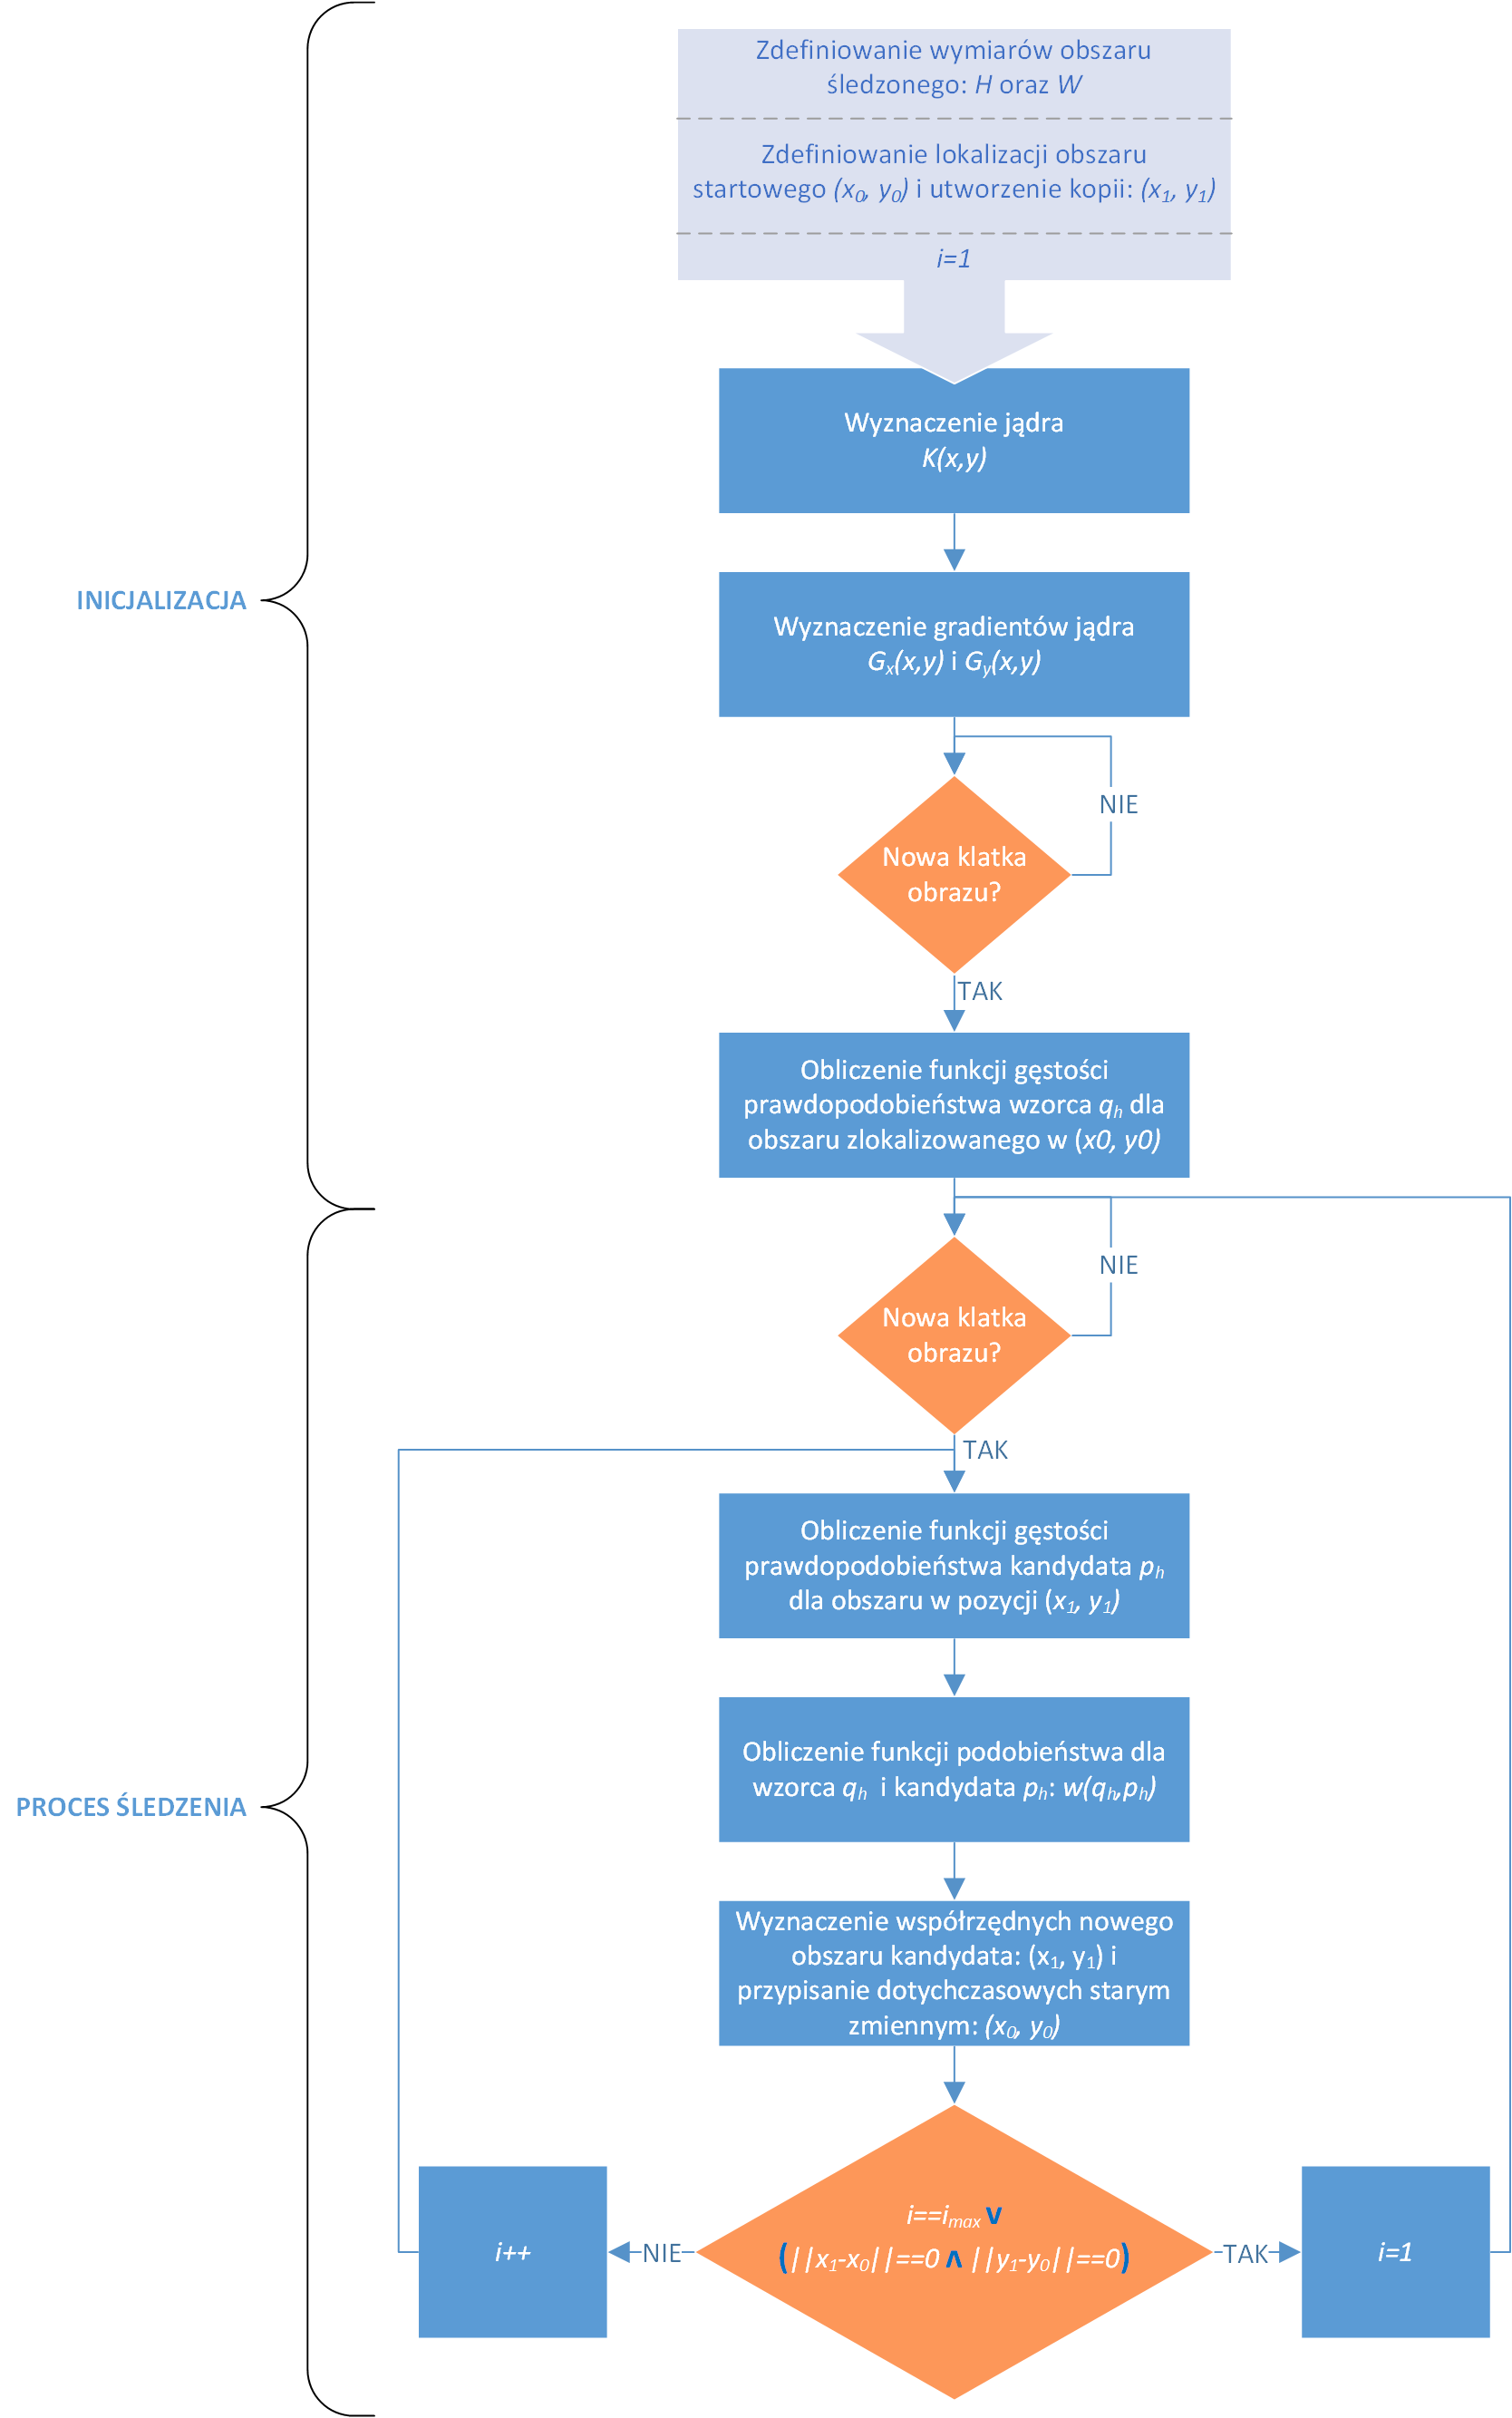
\includegraphics[width=14.5cm]{2_MS_visio.png}
	\caption{Schemat blokowy algorytmu MeanShift}
	\label{fig:MS_scheme}
\end{figure}
\subsection{Warunki zakończenia algorytmu}

W przypadku algorytmu iteracyjnego konieczne jest zdefiniowanie celów, które należy osiągnąć. 
Uzyskanie całkowitego podobieństwa pomiędzy wzorcem i kandydatem w zmiennej sekwencji obrazów jest w realnych warunkach nie do uzyskania.
Chcąc przetwarzać obraz w~czasie rzeczywistym, należy zakończyć przetwarzanie klatki przed momentem, w którym dane z następnej będą gotowe. 
Stąd dwa podstawowe warunki zakończenia algorytmu to:
\begin{enumerate}
	\item numer iteracji == maksymalna liczba iteracji
	\item $||P_{n_m}-P_{n_{m-1}}||<\epsilon$, 
\end{enumerate} 
gdzie: $n$ jest liczbą porządkową klatki, $m$ numerem iteracji algorytmu MeanShift dla konkretnej klatki, a $\epsilon$ stanowi akceptowalnie małą wartość.
W momencie spełnienia jednego z powyższych warunków, akceptuje się dotychczasowo uzyskaną zmianę położenia obszaru detekcji i~rozpoczyna obliczenia następnej klatki. 
Rysunek \ref{fig:MS_scheme} przedstawia schemat blokowy algorytmu MeanShift dla sygnału wideo. %TODO schemat blokowy %ODP OK
%TODO coś nie tak z ]ref / label %ODP OK




\section{Algorytm HOG+SVM}
\label{sec:HOG&SVM}

Jedną z metod śledzenia przez detekcję jest algorytm wykorzystujący zestaw cech obrazu -- konkretnie histogram zorientowanych gradientów (ang. \textit{Histogram of Oriented Gradients - HOG}); rolę decyzyjną pełni klasyfikator nazywany maszyną wektorów nośnych (ang. \textit{Support Vector Machine - SVM}).
Pierwotnie, rozwiązanie to zostało przedstawione w pracy \cite{Dalal} z zastosowaniem w detekcji pieszych; po nieznacznych zmianach powinno ono osiągnąć dobre wyniki w realizowanym projekcie. 
Metodykę klasyfikacji w oparciu o zestaw cech można również zastosować do detekcji innych obiektów -- w szczególności takich, które charakteryzują się dość unikalnym układem krawędzi.

Założeniem metody HOG+SVM jest przedstawienie fragmentu wejściowego obrazu (okna detekcji) w formie tzw. deskryptora -- wektora cech, który podlegać będzie klasyfikacji.
Proces generowania deskryptora polega na podzieleniu okna detekcji na mniejsze, jednakowej wielkości obszary (komórki). 
Dla każdego z pikseli wewnątrz okna obliczana jest wartość gradientu, jego orientacja i moduł, po czym piksele przydzielone do jednej komórki tworzą histogram zorientowanych gradientów. 
Okno detekcji jest następnie reorganizowane w formę bloków składających się z współdzielonych pomiędzy sobą 4 komórek (histogramów). 
Każdy z bloków jest niezależnie normalizowany, po czym wszystkie łączone są w postać wektora cech.

Klasyfikator SVM działa w oparciu o współczynniki otrzymane na etapie uczenia. Proces uczenia maszyny wektorów nośnych polega na wyznaczeniu hiperpłaszczyzny, która rozdzieli deskryptory należące do dwóch klas z maksymalnym marginesem. Wymaga to obliczenia zbioru wektorów cech na oknach detekcji, które zostały już przyporządkowane poszczególnym klasom.
Klasyfikacja jest etapem prostszym, w trakcie którego obliczana jest pozycja analizowanego wektora cech względem zdefiniowanej hiperpłaszczyzny (na tej podstawie określana jest jego klasa).
 %TODO 2 jakies to zamotane. Wejściem jest fargment tobarzu, dla niego wyliczane są cechy.... Zbiór wektroów cech + etykiety do SVM. %ODP OK
%TODO 2 było \new line -> unikać. %ODP OK



%TODO 2 też jeszcze raz przeczytać i wygładzić ten opisa. %ODP OK

\subsection{Konwersja RGB->GRAY i obliczenie orientacji} 
\label{sec:HOGgrad}
Pierwszym etapem jest dostosowanie pierwotnej palety barw RGB do 8-bitowej skali szarości. 
Dokonuje się tego, przekształcając każdy piksel według wzoru:
\begin{equation}
\label{eq:rgb2gray}
P_{GRAY}=0.299P_R + 0.587P_G + 0.114P_B 
\end{equation}
%Sumowanie się współczynników do jedności ma w zamierzeniu ograniczyć wynik tego przekształcenia do zakresu 0-255. %TODO zdanie niepotrzebne %ODP OK


Następnie przeprowadzana jest operacja kontekstowa w celu obliczenia gradientów kierunkowych $g_x$ oraz $g_y$; używane maski to odpowiednio: $[-1,0,1]$ oraz $[-1,0,1]^T$. 
Mając gradienty, dla każdego piksela (o koordynatach [$i,j$]) obliczany jest moduł i kąt ze wzorów:

\begin{equation}
\label{eq:HOGangles}
\left.\begin{aligned}
m(i,j)=\sqrt{g_x(i,j)^2+g_y(i,j)^2} \\
\theta(i,j)=arctg\bigg(\frac{g_y(i,j)}{g_x(i,j)}\bigg)
\end{aligned}\right.
\end{equation}

\subsection{Histogram gradientów}

W kolejnym etapie poddawany przetwarzaniu obraz jest dzielony na kwadratowe obszary (dla jasności nazywane od teraz \textit{komórkami}) o wymiarach $4\times4$, $8\times8$ lub $16\times16$ pikseli. 
W każdej z komórek zostanie wyliczony niezależny histogram na podstawie orientacji gradientu.
Oprócz rozmiaru komórki, kluczowym okazuje się również drugi parametr, czyli liczba przedziałów pojedynczego histogramu -- w tym wypadku zdecydowano, by rozpatrywany kąt przyporządkowywać jednemu z 9 przedziałów określających kierunek (z pominięciem zwrotu). Dzielą one równo zakres kątów $[0^{\circ},180^{\circ})$ -- i odpowiednio $[-180^{\circ},0^{\circ})$. 
Wynika z tego, że każdy kolejny fragment o szerokości $a=180^{\circ}/9=20^{\circ}$ będzie stanowić osobny przedział histogramu.

O ile typowy histogram tworzony jest poprzez inkrementację odpowiedniego licznika dla przedziału o 1, to tworzona struktura będzie wykorzystywać obliczony wcześniej moduł z gradientu. 
Dodatkowo, autorzy publikacji wspominają o możliwości interpolacji pomiędzy dwoma sąsiednimi przedziałami i inkrementacji poszczególnych wartości o proporcjonalne części modułu -- dowiedziono eksperymentalnie, że takie działanie pozytywnie wpływa na wyniki detekcji. 
Jeśli zatem przyjąć, że $\theta_h$ i $\theta_l$ to wartości kątów będących środkami dwóch sąsiadujących ze sobą przedziałów, którym jednocześnie najbliżej do badanego kąta $\theta$, wówczas będzie można zdefiniować elementy $M_h$ i $M_l$ jako: 

\begin{equation}
\label{eq:HOG_linear}
\left.\begin{aligned}
M_h(i,j)&=m(i,j)\bigg(\frac{\theta-\theta_l}{a}\bigg)\\
M_l(i,j)&=m(i,j)\bigg(\frac{\theta_h-\theta}{a}\bigg)
\end{aligned}\right.
\end{equation}

Ostatecznie, następuje powiększenie wartości dwóch odpowiednich przedziałów histogramu $H$ tworzonego w obrębie komórki zawierającej piksel o współrzędnych $(i,j)$:

\begin{equation}
\label{eq:HOG_increment}
\left.\begin{aligned} 
H(\theta_h,i,j)&=H(\theta_h)+M_h(i,j) \\ 
H(\theta_l,i,j)&=H(\theta_l)+M_l(i,j)
\end{aligned}\right.
\end{equation}

Koncepcję zilustrowano na rysunku \ref{fig:HOG_interpolation}.  
Przedstawia on okrąg z ponumerowanymi przedziałami, każdy o szerokości $a$. 
Jeśli orientacja obliczonego gradientu jest reprezentowana przez kąt $\theta=57^{\circ}$, to przedziałami uwzględnionymi w interpolacji będą te najbliższe, o numerach $3$ oraz $4$. 
Bazując na wartości kątów w ich środkach, $\theta_h$ i $\theta_l$, obliczane zostaną $M_h$ i $M_l$, jako odpowiednio: $35\%$ i $65\%$ wartości modułu zgodnie z wzorami \eqref{eq:HOG_linear}.
Wyjątkowym zdarzeniem jest takie, w którym kąt $\theta$ będzie znajdował w okolicy kąta $0^{\circ}=360^{\circ}$ (z przedziałami 1 oraz 9). 
Wówczas, dla wygody, w równaniach \eqref{eq:HOG_linear} należy użyć kątów $\theta_l=350^{\circ}$ oraz $\theta_h=370^{\circ}$.

\begin{figure}[h]
	\centering
	\hspace*{1cm}
	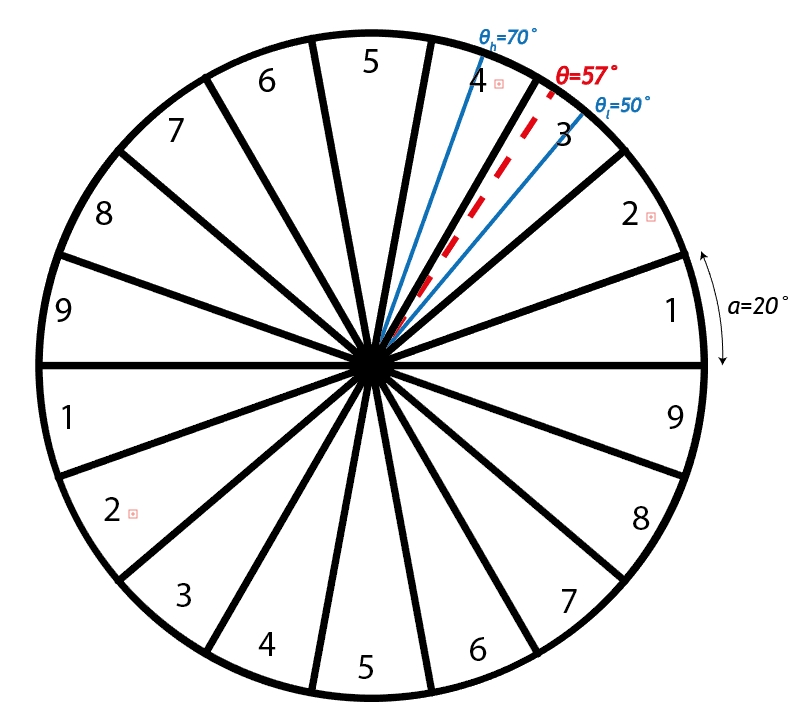
\includegraphics[width=12cm]{2_HOG_interpolation.jpg}
	\caption{Przykładowy problem liniowej interpolacji}
	\label{fig:HOG_interpolation}
\end{figure}

\subsection{Normalizacja}

Zazwyczaj, analizowany materiał wideo będzie rejestrowany w warunkach, w których ciężko zagwarantować równomierny poziom oświetlenia poszczególnych fragmentów obrazu.
Zakłócenia te negatywnie wpływają na wyniki działania algorytmu.
Z tego powodu proponuje się stosowanie normalizacji blokowej. 

Podejście zakłada utworzenie struktur nazywanych \textit{blokami}, gdzie każdy z nich obejmować ma $2 \times 2$ sąsiednie komórki. 
Dla obrazu, na bazie którego utworzono $N \times M$ komórek, powinno powstać $(N-1) \times(M-1)$ bloków -- przy ich generowaniu wykonuje się krok o jedną komórkę w poziomie i/lub w pionie względem poprzedniego obszaru. 
Rozmiar pojedynczego bloku sugeruje, że będzie się on składał z 4 histogramów, w formie wektora: 
\begin{equation}
v=[H_{i,j}, H_{i,j+1}, H_{i+1,j}, H_{i+1,j+1}],
\end{equation} 
gdzie: $i$  wiersz, $j$ - kolumna. Następnie należy dokonać normalizacji, wykorzystując jedną z~ sugerowanych zależności: 

\begin{equation}
\label{eq:HOG_norm1}
\left.\begin{aligned} 
L1&=\frac{v}{\sum_{i}^{n}v_i+\epsilon}
\end{aligned}\right.
\end{equation}

\begin{equation}
\label{eq:HOG_norm2}
\left.\begin{aligned} 
L1_{sqrt}&=\frac{v}{\sqrt{\sum_{i}^{n}v_i+\epsilon}}
\end{aligned}\right.
\end{equation}

\begin{equation}
\label{eq:HOG_norm3}
\left.\begin{aligned} 
L2&=\frac{v}{\sqrt{\sum_{i}^{n}v_i^2+\epsilon^2}}
\end{aligned}\right.
\end{equation}

\begin{equation}
\label{eq:HOG_norm4}
\left.\begin{aligned} 
L2_{hys}&=\frac{v}{\sqrt{\sum_{i}^{n}v_i^2+\epsilon^2}}, v\leq 0.2
\end{aligned}\right.
\end{equation}
W powyższych równaniach $\epsilon$ to stała o małej wartości, a $n$ to liczba elementów w bloku (4 histogramy po 9 przedziałów $\rightarrow$ 36). Wektory $L$ zebrane z całego okna detekcji budują ostateczny wektor cech, na którym pracować będzie klasyfikator.

Niech podsumowaniem rozważania będzie przykład -- okno detekcji o rozmiarze \mbox{$200\times 400$} i komórka o wielkości $8 \times 8$. 
Wynikiem opisywanej procedury będzie utworzenie aż \mbox{$25\cdot50=1250$}~komórek i $24\cdot 49=1176$ bloków. 
Po normalizacji blokowej klasyfikator otrzymałby aż $1176\cdot4\cdot9=42336$ wartości do przetworzenia. 
Obsługa tak dużej ilości danych niosłaby za sobą konieczność pewnych optymalizacji, co będzie rozważone w rozdziale poświęconym implementacji algorytmu.
%TODO przykłąd nietafiony, bo zawsze się wykonuje detekcję w oknach %ODP wielkość zmieniono, chodziło mi raczej o przejście przez obliczenia na jakimkolwiek przykładzie.
%TODO 2 to dlaczego nie wybrał Pan std. tj. 128 x 64. %ODP przykład dużego okna detekcji pokazuje jak wiele elementów należałoby przetworzyć, co też uzasadnia wykorzystanie okna 128x64. Poza tym, jeśli ktoś chciałby się oprzeć na pracy i implementować HOG+SVM, to ma dwa przykłady obliczeń - ten którego używam, i ten powyżej

\subsection{Klasyfikator SVM}

Maszyna wektorów nośnych to klasyfikator binarny, który dzięki swej prostocie i skuteczności jest powszechnie wykorzystywany w procesie odróżniania klas w różnych aplikacjach, w~tym wizyjnych \cite{Gunn}. 
Jego działanie tradycyjnie można podzielić na dwie fazy: uczenie i klasyfikację. 
Etap uczenia to relatywnie dłuższy czasowo proces wyznaczenia hiperpłaszczyzny, która z jak najlepszym marginesem rozdzieli wejściowe wektory cech obiektów klasyfikowanych jako \textit{1} od tych określonych jako \textit{0} (umownie). 
Stosowane podeście nie powinno odbiegać od klasycznej metodologii uczenia maszynowego -- dysponując zbiorem danych wejściowych, należy dokonać podziału na próbki uczące oraz testowe (w stosunku około 70:30).
Każdy z~tych podzbiorów (a przede wszystkim uczący) powinien posiadać zarówno obiekty zdefiniowane jako pozytywne, jak i negatywne. 
W niniejszej pracy, która ma na celu rozpoznanie osoby w postawie stojącej, wymagane będzie użycie obrazów o rozmiarach $128 \times 64$ pikseli, przedstawiających taką postać w jak największej liczbie kombinacji (ale w podobnej skali), lecz także obrazów ze zróżnicowaną scenerią, na których żadnych osób jednak nie ma. 
Dla poprawienia ostatecznych wyników należy zadbać również o zróżnicowanie obrazów pod kątem poziomu oświetlenia, a nawet tła otaczającego postać.
Etapem klasyfikacji nazwać można wykorzystanie otrzymanych w procesie uczenia parametrów do wyznaczenia położenia badanego wektora cech względem hiperpłaszczyzny. 
Na tej podstawie do obiektu zostanie przydzielona odpowiednia klasa.

\subsubsection{Uczenie}

Aby detektor mógł działać poprawnie, klasyfikator musi dysponować odpowiednimi parametrami. 
Uzyskuje się je na etapie uczenia, używając odpowiedniego zestawu danych.
Wzorując się na pracy Dalala oraz Triggsa, postanowiono skorzystać ze zbioru ponad 5000 obrazów udostępnionych przez twórców. 
Specyfikacja tego zestawu pozwala nauczyć klasyfikator rozpoznawania osoby na obrazie o wielkości $128 \times 64$ pikseli. 
Wysokość przedstawionej osoby, wyrażona w pikselach, powinna oscylować wokół 95 ($\pm$ 5). 
Zgodnie z przyjętą metodologią, zestaw ten zawiera gotowy podział na próbki pozytywne i negatywne, dalej pogrupowane na zestaw uczący oraz testowy w stosunku zbliżonym do 70:30. 
Przykłady przedstawiono na ilustracji:

\begin{figure}[h]
	\centering
	\captionsetup{justification=centering,margin=1cm}
	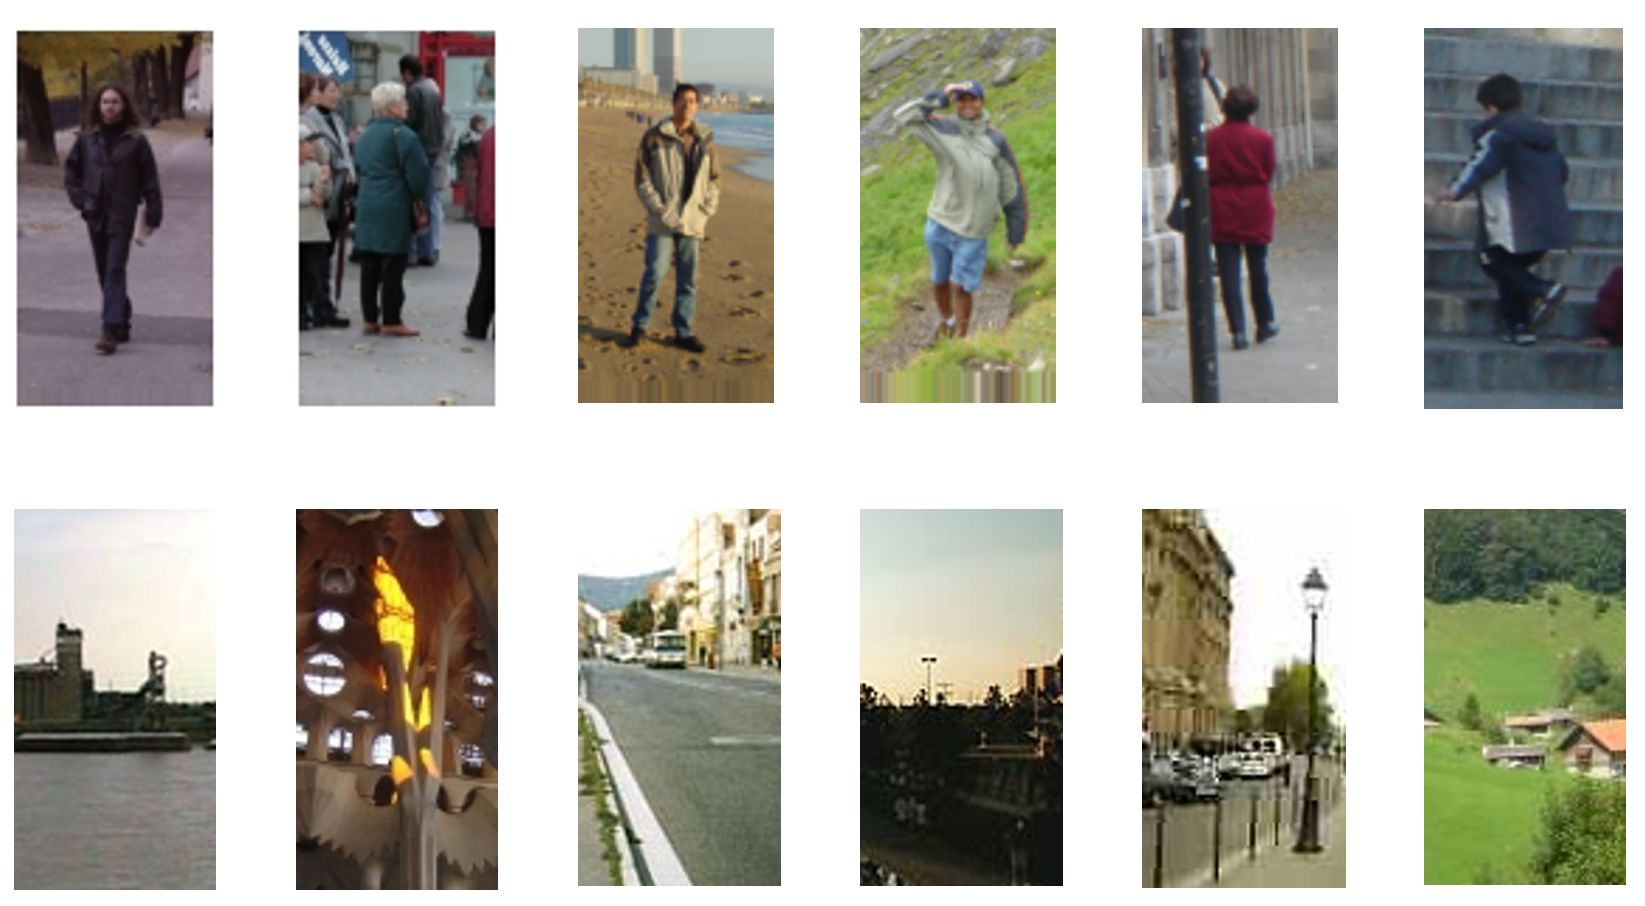
\includegraphics[width=14.5cm]{2_HOG_image_examples.jpg}
	\caption{Przykłady obrazów ze zbioru wykorzystanego przy uczeniu -- na górze próbki pozytywne, na dole negatywne}
	\label{fig:HOG_image_examples}
\end{figure}

Wśród próbek pozytywnych połowa plików to duplikaty odwrócone horyzontalnie. 
Ma to zapewnić poprawne uwzględnienie cech osób niezależnie od orientacji względem kamery.

\subsubsection{Klasyfikacja}
\label{sec:klasyfikacja}
Etap ten jest stosunkowo prosty i stanowi główną zaletę klasyfikatora SVM. 
Wymaga bowiem wcześniejszego przeprowadzenia etapu uczenia oraz dostarczenia wektora cech klasyfikowanego obiektu. 
Obliczane jest wówczas równanie:
\begin{equation}
\label{eq:HOG_classification}
\left.\begin{aligned} 
r=\sum_{i=1}^{N}(a_i\cdot l_i)+b,
\end{aligned}\right.
\end{equation}
gdzie: $l_i$ to elementy wektora cech, natomiast $a_i$ i $b$ to parametry wyliczone na etapie uczenia. 

W projekcie, proces uczenia i klasyfikacji oparto o funkcje dostępne w środowisku \mbox{MATLAB}, gdzie to równanie jest nieco zmodyfikowane:
\begin{equation}
\label{eq:HOG_classificationMATLAB}
\left.\begin{aligned} 
r=-\sum_{i=1}^{N}a_i(l_i+b_i)-c,
\end{aligned}\right.
\end{equation}
gdzie: $a$, $b$ oraz $c$ to parametry hiperpłaszczyzny wyliczone na etapie uczenia ($a$ i $b$ -- wektory, $c$ -- skalar).

Dla obu przypadków, detekcja wskazuje obiekt jako przynależący klasy jeśli $r>0$, w~przeciwnym wypadku go odrzuca.


\subsection{Detekcja na ramce sekwencji wideo}

Omówiony klasyfikator jest w stanie rozpoznać postać znajdującą się w centrum próbki o~rozmiarze $128 \times 64$ pikseli. 

Wykonie detekcji na obrazie o dowolnym rozmiarze np. $1280 \times 720$ wymaga zastosowania mechanizmu okna przesuwnego. 
Dysponując określonym obszarem zainteresowań, algorytm powinien sprawdzić każdą możliwą konfigurację położenia okna $128\times 64$ wewnątrz tego obszaru. 
Przykładowo oznacza to przesuwanie okna o 1 piksel w bok, a po dotarciu do prawej linii -- o 1 piksel w dół.
Takie podejście skutkuje bardzo dużą złożonością obliczeniową -- dla obszaru zainteresowań o wymiarach $144\times 96$ i rozpatrywanego okna istnieje 512 możliwości (512 wektorów cech). 
W praktyce zwiększa się wykonywany krok o kilka lub kilkanaście pikseli -- dla obrazu o dość dużej rozdzielczości $1280 \times 720$ jest to akceptowalny poziom pominięcia niektórych szczegółów.
Przykład realizacji okna przesuwnego jest przedstawiony na rysunku \ref{fig:HOG_mesh}.
%TODO 2 może tu odnieść to do tego 1280 x 720 %ODP OK

%TODO 2 Może jednak rysunek poglądaowy jak to okno działa. %ODP OK

Metoda HOG+SVM jest mało odporna na zmianę wielkości wykrywanego obiektu na oryginalnym obrazie, a porównując wymiary ramki ($1280\times 720$) z wielkością okna detekcji, może wydawać się to poważnym ograniczeniem. 
Skutecznym rozwiązaniem okazuje się być zastosowanie algorytmu HOG+SVM na kilku kopiach obrazu z różnym współczynnikiem skalowania. %TODO 2 to w rózny sposób sugeruje, że innym algorytmem.... a to nie o to chodzi. %ODP OK
Metodyka detekcji w wielu skalach stanowi dobrą odpowiedź na jedno z założeń systemu, mówiące o konieczności określenia odległości kamery od rozpoznanej osoby, by poprzez odpowiednie sterowanie utrzymać zadany dystans.  %TODO z tym kierunkiem ? -> niejasne %ODP OK
Z każdej skali należy wydobyć próbki obrazów o wymiarach $128\times 64$ i znaleźć najlepszą pozytywną detekcję. 
Opisują to rysunki \ref{fig:HOG_scaling}. 
\begin{figure}[h]
	\centering
	\captionsetup{justification=centering,margin=1cm}
	\hspace*{0cm}
	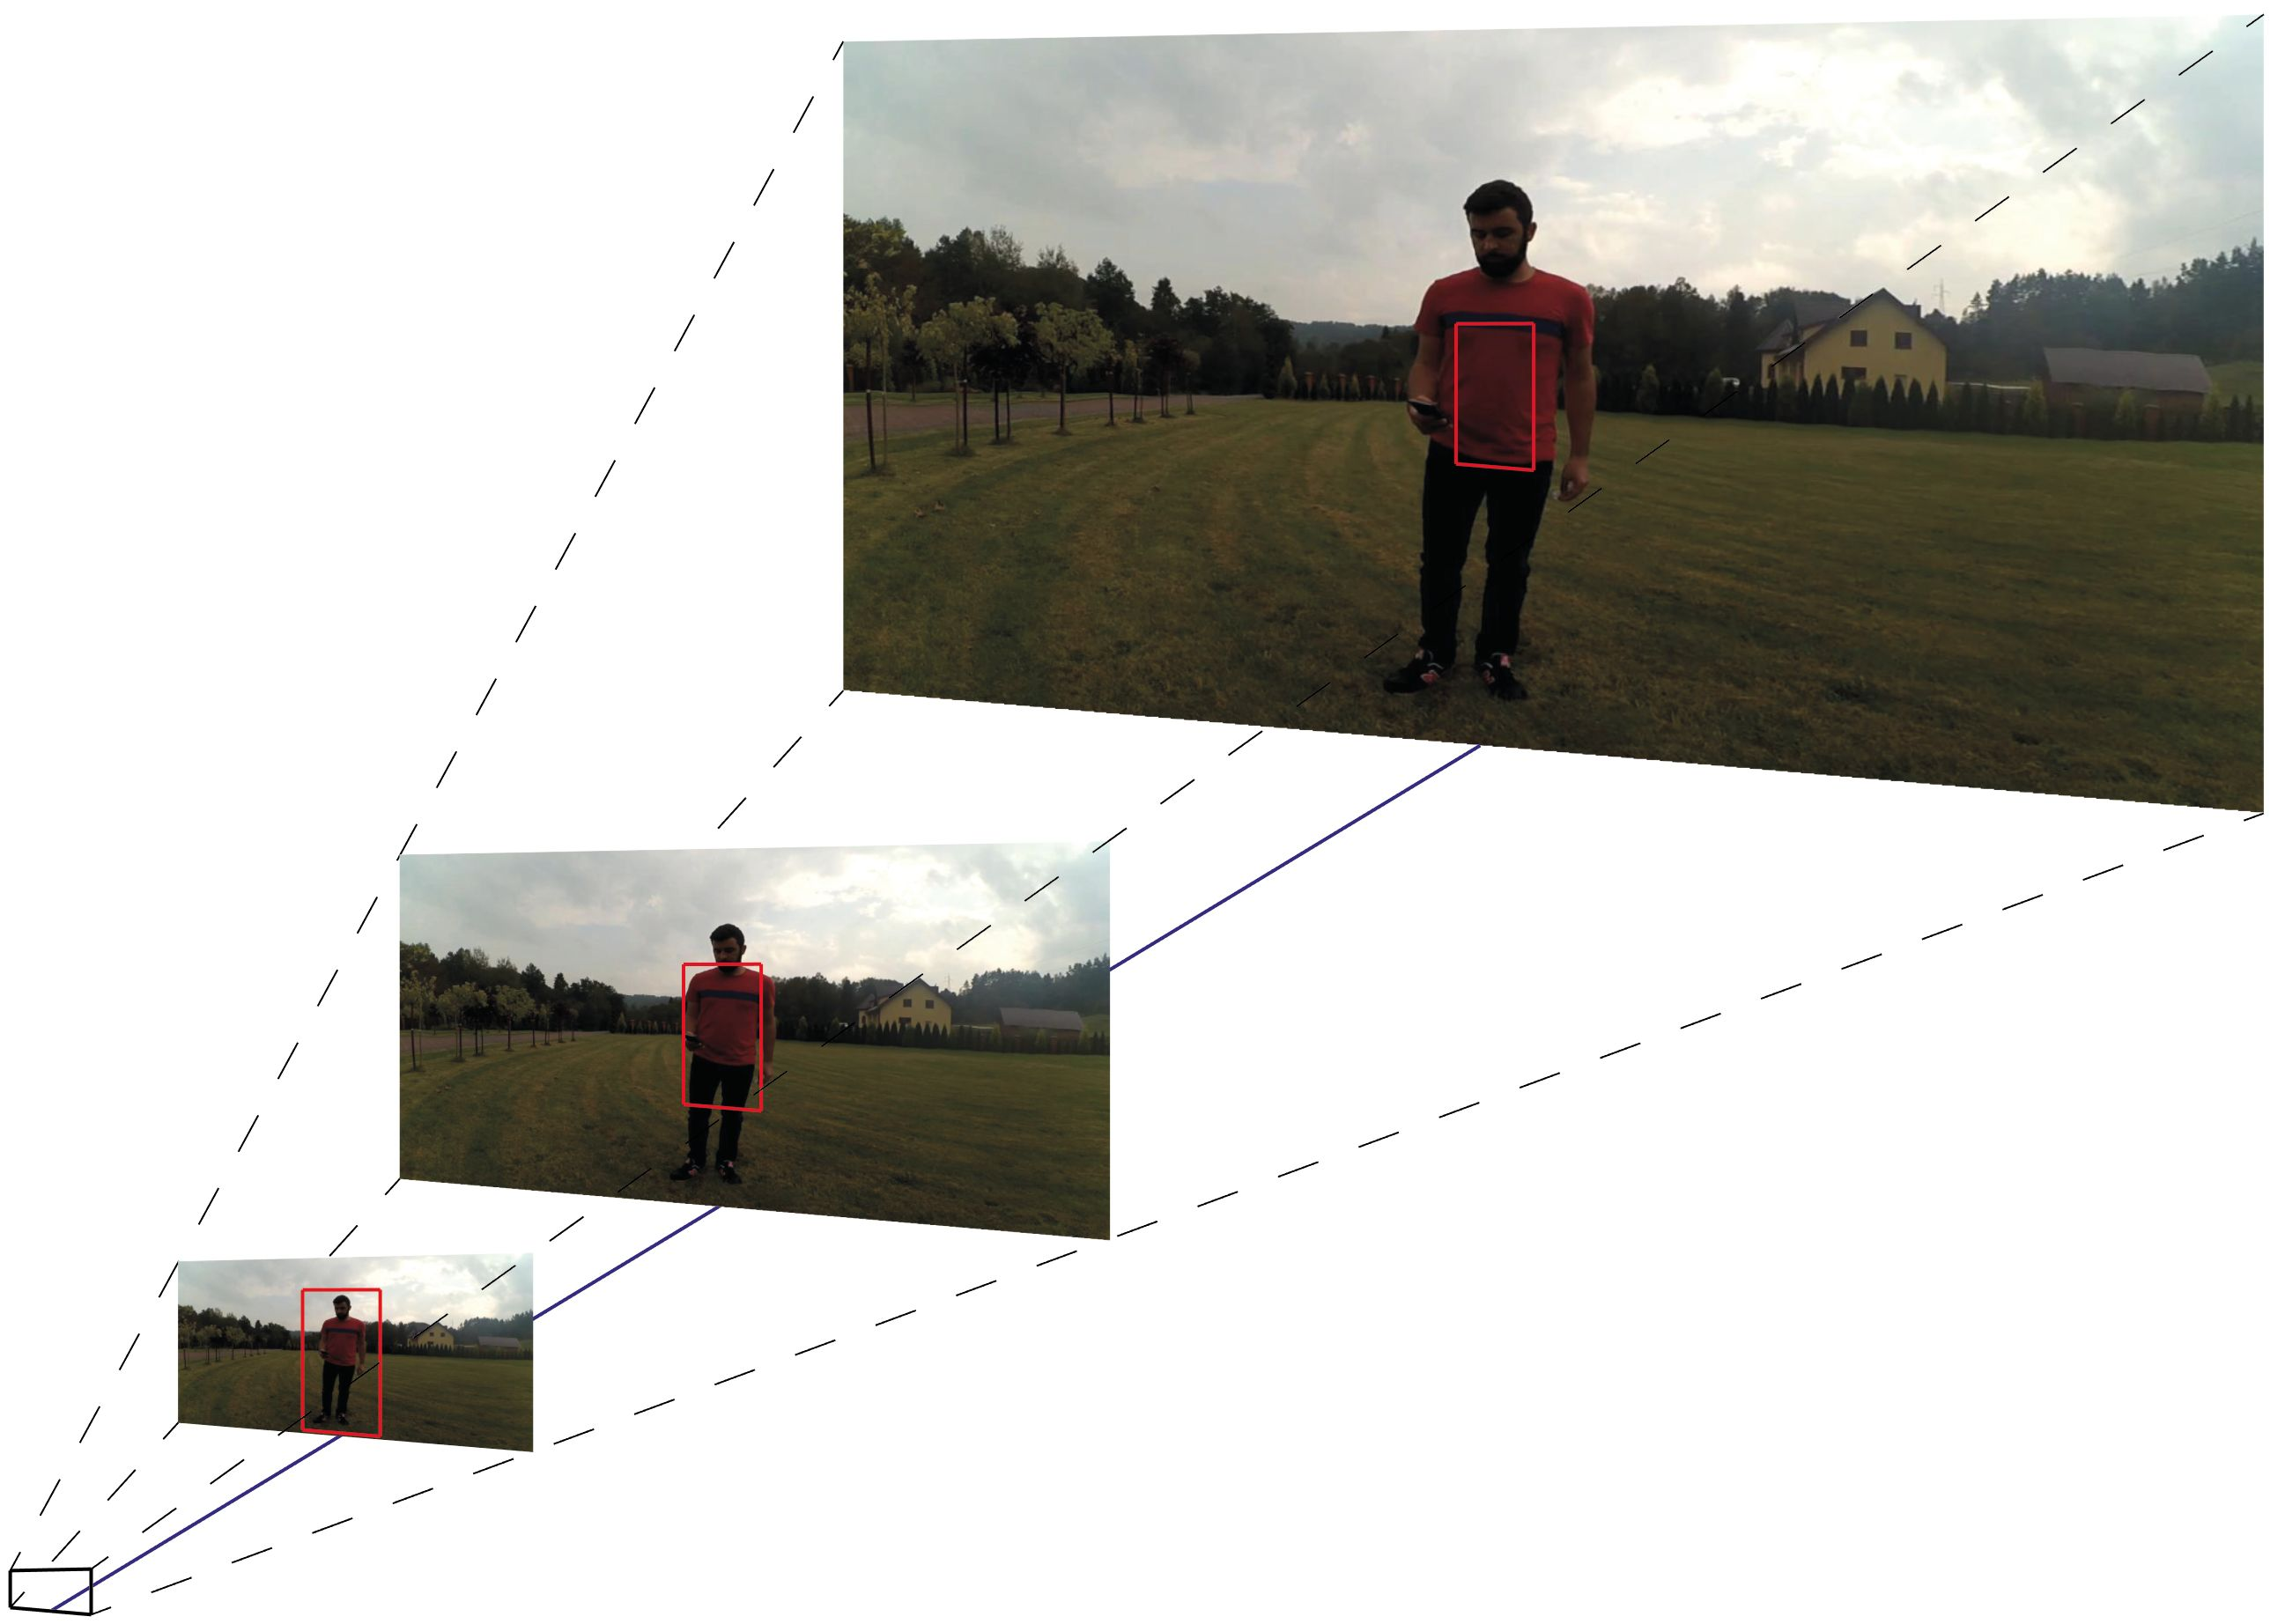
\includegraphics[width=15.5cm]{2_scaling.jpg}
	\caption{Skalowanie 1:1, 1:2 oraz 1:4 z naniesionym przykładowym oknem detekcji $128 \times 64$}
	\label{fig:HOG_scaling}
\end{figure}

Po zakończeniu klasyfikacji dla wszystkich skal następuje grupowanie wyników -- w efekcie wyłaniane jest najlepiej sklasyfikowane okno i określana jest jego pozycja na oryginalnym obrazie. 
W~przypadku przedstawionym na rysunku, klasyfikator prawdopodobnie rozpozna postać na oknie detekcji z obrazu przeskalowanego w stosunku 1:4. Stała wielkość okna detekcji $128\times 64$ każe wnioskować, że osoba wykryta na oryginalnym obrazie mogłaby być znacząco oddalona od kamery. Znając przybliżoną odległość pomiędzy kamerą tak wykrytą osobą i stosując proste twierdzenie Talesa, można oszacować jej rzeczywistą odległość dla pozytywnej detekcji w jednej ze skal. 
Opisuje to poniższy wzór:
\begin{equation}
\label{eq:scaling}
d_r=\frac{d_o}{s_c},
\end{equation}
gdzie: $d_r$ to aktualna odległość pomiędzy osobą i kamerą , $d_o$ to odległość do wykrytej osoby na obrazie oryginalnym (zmierzona), a $s_c$ to skala obrazu (w postaci ułamkowej), w którym okno detekcji uzyskało najlepszy wynik.

Szczegóły realizacji algorytmu opisano w podrozdziale \ref{HOG_SVM_realization}.


%TODO tu komplemetnie brakuje  opisu jak działa tzw. okno przesuwne.  Same skale też można lepiej opisać. %ODP Dodano opis, w rozdziale o implementacji jest o tym więcej napisane
%TODO Kolejna sprawa to tzw. grupowienie detekcji z wielu skal. %ODP to mam opisane w implementacji 



%TODO 2 skoro tak to napisać, że szczegóły pzredstawiono w jakimś tam rozdziale. A o tym grupowaniu to chociaż wspomnieć i \ref %ODP OK
